% This is samplepaper.tex, a sample chapter demonstrating the
% LLNCS macro package for Springer Computer Science proceedings;
% Version 2.20 of 2017/10/04
%
\documentclass[runningheads]{llncs}
%
\usepackage{graphicx}
\usepackage[dvipsnames]{xcolor}
% Used for displaying a sample figure. If possible, figure files should
% be included in EPS format.
%
% If you use the hyperref package, please uncomment the following line
% to display URLs in blue roman font according to Springer's eBook style:
% \renewcommand\UrlFont{\color{blue}\rmfamily}

\begin{document}
%
\title{Literary Studies Meet Corpus Linguistics: Estonian Pilot Project of Private Letters in KORP\thanks{Supported by the institutional research grant “Formal and Informal Networks of Literature, Based on Sources of Cultural History” (IRG22-2, Estonian Ministry of Education and Research),  and related to the Centre of Excellence in Estonian Studies (CEES, European Regional Development Fund).  Development of KORP and adding corpora in Estonian is supported by the ERDF project The Federated Content Search for the Center of Estonian Language Resources'' (2014--2020.4.01.16--0134) under the activity ``Support for Research Infrastructures of National Importance, Roadmap''.  Research is supported by the ASTRA (2014-2020.4.01.16-0026) and the Center of Excellence for Estonian Studies via the European Regional Development Fund (TK145).}}
%
\titlerunning{Private Letters in KORP}
% If the paper title is too long for the running head, you can set
% an abbreviated paper title here
%
\author{Marin Laak\inst{1} \and Kaarel Veskis\inst{1} \and\\
Olga Gerassimenko\inst{2} \and Neeme Kahusk\inst{2} \and
Kadri Vider\inst{2}}
%
\authorrunning{M. Laak et al.}
% First names are abbreviated in the running head.
% If there are more than two authors, 'et al.' is used.
%
\institute{Estonian Literary Museum\\
  Vanemuise 42, 51003 Tartu, Estonia\\
\email{\{marin.laak,kaarel.veskis\}@kirmus.ee}\and
Institute of Computer Science, University of Tartu,\\
J. Liivi 2, 50409 Tartu, Estonia
\email{\{olga.gerassimenko,neeme.kahusk,kadri.vider\}@ut.ee}
}
%
\maketitle              % typeset the header of the contribution
%
\begin{abstract}
  Digitisation of cultural heritage in Estonia has been in progress during recent years, and we will see expansive mass digitalisation of printed books and handwritten dokuments in the very near future.
  
  This situation and potential actualises the questions of the usage of the literary heritage. In our paper, we consider the benefits for the digital literary research that arise from representing a literary text collection as a linguistically annotated language resource. We discuss the pilot project of creating a DH corpus based on private letters between two avangardist writers  Johannes Semper and Johannes Barbarus during the first Estonian Republic in the beginning of the 20th century.
  
The advantages and possibilities of corpus search system KORP that we have chosen for representing and searching literary heritage DH corpora as a language resource are described. Challenges that application of Natural Language Processing and Text and Data Mining imposes on the preparation and representation of the texts are discussed along with the benefits for the research. 


\keywords{literary studies \and private letters \and digital heritage collections \and corpus linguistics \and data mining \and natural language processing}

\end{abstract}
%
%
%
\section{Introduction}

The application of Language Technology (LT) and Text and Data Mining (TDM) methods and tools is gradually increasing and becoming more relevant in Estonia. Similarly to the Nordic and Baltic countries, Estonia can expect an explosive growth of digital heritage and text resources: preparations for massive digitisation of cultural heritage started in 2019 as national programme. The creation of these new digital resources will be the priority for all Estonian leading memory institutions and the scope of this huge project includes all different types of cultural heritage (printed books, archival documents, photo and film heritage, ethnographic and fine art objects) [5, 9] Digitized resources will be made accessible on the Internet as open data, but it is still an open question how and for what purpose can such digital resources be used \cite{laakviires}. 

What are the new challenges and the new knowledge offered by using the applications of Linguistic Analysis tools in analysing the digital literary heritage? Our interdisciplinary project “Literary Studies Meet Corpus Linguistics” concentrates on using cultural heritage, especially literary history sources in research with the help of the LT\&TDM methods. The primary question is how to bridge the gap between the research possibilities offered by the contemporary LT\&TDM and the ever increasing resources of texts and other digital data, produced by memory institutions. This has proved to be a complicated task and international practice has shown that literary scholars are slower to embrace new practices than linguists for whom corpus-based research is already a professional standard. In general, literary scholars are used to working with texts with traditional methods, analysing them as undivided poetical and semantic entities \cite{viireslaak18}. Digitizing of texts often preserves them as undivided and unannotated entities with occasionally added metadata - as a result, the digitized materials are human-readable rather than machine-readable.

LT\&TDM methods require treating literary works or texts as data, which can be analysed and processed with computer programmes. To research for statistics and trends in the data, a literary scholar needs either to do a close reading of literary texts as huge data amounts, or to develop new professional skills in data analysis methods. This imposes rethinking the approach to empirical object in literary studies in general and posing new and different research questions. The possibility to compare text strategies, rhetorical and stylistic patterns in literary, religious and political text corpora might give us new insights into intertwining ideology, rhetoric and identity presentations. One of the important trends of automated textual analysis in DH is Sentiment Analysis which, for instance, allows to measure emotion in parliamentary debates \cite{Rheault2016}.


\section{Private letters as a literary source}

The empirical base of our pilot project of private letters in KORP is based on the archival ego-documents. This is a rare collection of handwritten private letters: the correspondence between two Estonian writers Johannes Semper (1892–1970) and Johannes Barbarus (1890–1946). The authors were well-known avant-garde writers in Estonian literature, best friends and school classmates. They shared the same intellectual attitudes, views, and values. For example, they were Francophiles and during several decades they both mediated and translated French literature into Estonian. 

During the years covered by the correspondence, in 1911-1939, Barbarus published the total of 17 collections of poetry, and Semper published four collections of poetry and four books of short stories and novels. The letters were written mainly in different places in Estonia, and also during travels: they both travelled extensively in Europe (and other parts of the world) and in their letters they described to each other the sights they saw as well as the literary events at home. They also wrote about their work, everyday life, health and prescriptions, hobbies (hunting, swimming, skating, etc.), and guests. 

The temporal and contextual frames of this correspondence is the period in Europe between two World Wars and, according to French philosopher Pierre Bourdieu, the creation of  the Estonian ‘cultural field’ in the Estonian Republic in years 1918-1940. As such, the correspondence offers semantically rich and multidimensional content for literary scholars.  

Generally, we are inspired by the question how this kind of sources (private letters, correspondences, manuscripts, etc.) in different kinds of computer-readable formats (pdf, docx, txt etc.) can be used for creating new knowledge in the interdisciplinary field of literary studies, including biographics and life writing studies \cite{2015}. 

The private correspondence of two Estonian writers during 28 years as an empirical material is extremely rich in the themes and possibilities to pose the traditional as well as the new research questions, e.g the factors of subjectivity and emotionality, verbal and poetic creativeness of the both authors.  

The original letters are held at different archives: the letters of Barbarus to Semper are at the Estonian Cultural History Archives of the Estonian Literary Museum and the letters of Semper to Barbarus are at the Estonian National Archives due to the unique literary and historical value of this correspondence. Their correspondence consists of 670 letters with, all in all, more than 1,100 pages and more than 310 890 tokens (249 970 words). 


\section{KORP as a tool for corpus linguistics}

KORP is a corpus query analysis system that allows to find concordances and build various statistics from differently annotated corpora using text metadata (author, year of publishing, text type etc) and linguistic annotation (splitting into sentences and words, punctuation, morphology, syntax and semantics). Technically, KORP is a frontend tool that uses much of IMS Open Corpus Workbench as backend. It was created and maintained at Swedish Language Bank Språkbanken \cite{BORIN12.248} and is being developed and customised by language technology networks in several countries: Sweden, Finland, Norway, Estonia, Denmark, Island and Italy (internal use in the University of Florence).  

Estonian KORP is hosted by the Centre of Estonian Language Resources. The Estonian data available for search in KORP currently consists of more than 850 million tokens. As Estonian is a highly inflective language with a rich morphology and free word order, almost all texts are automatically annotated and disambiguated on the morphological level to enable form- and baseform-based search.


As a pilot project for the needs of literary studies in addition to the corpora designed for linguistic research, we have added Correspondence Corpus of private letters (Semper and Barbarus, 1911-1940). The original handwritten manuscripts where already transformed to typewritten and then to electronic format; they had to be further transformed to a computer-readable text files by manually adding metadata and automatically analyzing and disambiguating morphological categories. 

KORP was chosen because of its open source value, search flexibility and easiness, graphical overview of search results in subcorpora, easy switching between concordances and broader context (as well as between statistics and concordances), broad possibilities to group search statistics and automatically created relative statistics (occurrences per million tokens).  The search results and statistics from the KORP are exportable to Comma Separated Values (CSV) format; we plan to extend the export to the Excel (XLS) and HTML formats (already used in Finnish KORP),  integrate a single sign-on access for corpora with restricted usage, introduce links to audio and video data, links to lexicons and automatic annotation of corpora, the features already implemented in KORP of the other countries (Finland, Sweden, Norway). Text fragments cited in KORP are limited to a sentence or a passage, so that KORP does not infringe copyrights; metadata cited in the query results allow exact pinpointing of the source of the sentence, and there is a possibility to link the whole texts hosted elsewhere to the search metadata for close reading of the broader context when needed. 


\section{Challenges for annotation in manuscript corpus}

The private letters of writers, the correspondence as whole was not meant for wider audience. Creators of the corpus met serious difficulties because often, both correspondents were very familiar with the subjects mentioned in the letters, so that sometimes they only hinted at the events or persons and used plenty of abbreviations known only to themselves. Which distinctive features of older correspondences need to be considered in preparing them to be used as corpus? Several steps are necessary to convert the digitised collection into a morphologically analysed language corpus, and to provide it with essential metadata about the sources.

\begin{enumerate}
\item The first step in digitising all kinds of texts, correspondences or published works, is the character recognition of the files or even the rewriting of the handwritten originals or typed text in the paper to the files; the latter is important in case of manuscripts. 

\item In order to enable statistics and to find different linguistic phenomena in the texts, it is important to tokenise at least sentences and words, and to preserve meaningful units (chapters, articles, verses, letters). 

  \item The process of annotation was carried on semi-automatically. At first stage, sentence boundaries were determined, then words were tokenised. Tokenised words were lemmatised and tagged by part-of-speech and other grammatical features.

\end{enumerate}

Different levels of annotation make it possible to search for different linguistic or other phenomena. In a tokenised text we can search by word forms (or their parts), but not by lemmas. In a lemmatised text we can search also by lemmas, but not by morphological characteristics (e.g., the case, the number). When the text has been morphologically analysed and disambiguated, we can search also by morphological characteristics and parts of speech. The automatic morphological analysis and automatic disambiguation that enable searching for different morphological forms of a word based on the lemma, seriously improve the usability and quality of the corpus. The accuracy of automatic morphological disambiguation in the Estonian standard language corpora reaches up to 93-98\% \cite{veskisliba}.  The accuracy for these texts is fare less.


The additional clause tokenisation helps to find the linguistic phenomena occurring in the clauses (e.g. the phrasal verbs and idiomatic expressions). The yield and accuracy of automated tokenisation of clauses in the Estonian standard language corpora is, respectively, 95\% and 96\% \cite{Kaalep2012}. Meaningful units, e.g., temporal expressions or named entities, found in the text can also be used in searches. If all the meanings of words were tagged, it would be possible to search for a specific meaning of a word and discard all other meanings. 

\section{Annotation types specific for private letters}

\subsection{Abbreviations}

In this corpus, there are a lot of nonstandard abbreviations that were comprehensible to the authors of the letters. They reflect both the historical period and the personal context and idiolects. Being avant-garde poets, Semper \& Barbarus both experimented with the language a lot. The abbreviations pose a challenge to the morphological analysis and disambiguation of abbreviations itself, but also of the neighbouring words, the disambiguated analysis of which often relies on the context (for instance, “is. Linde” should be analyzed as “master Linde” and not as a sentence ending and a starting of a new sentence although there is no common abbreviation “is.” in the standard Estonian). 

\subsection{Date and other temporal expressions}

The date format of the manuscript letters varies greatly: ``11. jaanuar 1927'', ``19/XII.37'', ``2. 2. 1934'', ``J\~oulu 3. p\"uhal 1934'' (on the 3rd holiday of Christmas 1934). The date in the format chosen by the letter authors needs to be saved as a part of the text, but in addition to that, all the date formats need to be normalized so that they could be present in the letter metadata in a standardized format (i.e., YYYY-MM-DD) whenever possible. When it is not possible, we can use the category “undefined” for the analysis transparency. Temporal expressions in the text of letters can be automatically recognized with the help of EstNLTK library for Python (https://github.com/estnltk/estnltk) and a software tool developed by Siim Orasmaa \cite{ORASMAA14.530}. 

\subsection{Named Entity Recognition}

Special interest for the literary scholars lies in the proper names used in the letters: their usage combined with the metadata (time period, author) might lead to recognizing the important patterns and tendencies. 

Named Entity Recognition (NER) annotations can be produced with the EstNLTK toolkit (https://github.com/estnltk/estnltk) and include the types of entities: person (PER), organisation (ORG), location (LOC) and timex (TIMEX). 

\subsection{Detect other languages}

Semper \& Barbarus were both promoters of French literature and culture in Estonia. They both worked as translators and travelled a lot. They scattered their letters with words, phrases, sentences and longer citations in many other languages than Estonian that were familiar to them (Latin, French, Russian, German). This is a challenge for the automatic language recognition and annotation tools which are currently oriented only to the analysis of standard Estonian. These tools does not help much in case of excerpts from other languages, but if such code-switching pieces were precisely recognized, lemmatized and analyzed, that information would be useful both to linguists and literary scholars.


\begin{figure}
  \centering
  \begin{minipage}{0.8\textwidth}
\itshape
  ``\colorbox{Green}{Bifur}''i kiri saabus \colorbox{Magenta}{Sinu kirjaga \"uhel p\"aeval}. Palutakse \colorbox{Magenta}{kohe} luule \"ule artikkel \"ara saata ja kedagi paluda, kes teisi k\"usimusi
  (\colorbox{Orange}{sur la vie en g\'en\'eral})
käsitaks. Neil olla t\~olkija, nii siis v\~oivat eesti keeleski kirjutada. Et mul artikkel juba valmis oli, siis saatsin ta \colorbox{Magenta}{t\"ana} minema. Kui Sul lusti midagi saata, siis l\"akita \colorbox{Magenta}{kohe} , --- ehk novelli t\~olge (maksavad 50 \colorbox{CornflowerBlue}{fr.} lehek\"uljest), ehk siis mahutavad neljandamasse \colorbox{CornflowerBlue}{nr}-isse; ehk viskad proosa \& teaatri \"ulegi artikli. Aadress : ``\colorbox{Green}{Bifur}'' , \colorbox{Green}{\'Editions du Carrefour} , \colorbox{Cyan}{199 , boul . St.-Germain , Paris} (VIe) (\colorbox{Orange}{M–eur le r\'edacteur en chef}  \colorbox{Green}{Ribemont Dessaignes}). K\"usisin kirjas, kas nende t\~olkija luuletisi t\~olkida v\~oiks, siis v\~oiksime valiku teha, ehk Suitsi ilmuva antoloogia neile saata. ``\colorbox{Green}{Bifur}'' harrastab k\"ull rohkem proosat \& informatsioonilaadilisi \"ulevaateid, nii siis vaevalt nad luule liimile l\"ahevad, aga eks ole ju veel teisi \v{z}urnaale p\"a\"ale ``\colorbox{Green}{Bifur}''i, kus avaldada saaks, kui aga t\~olkija leiduks. Mis teeb see \colorbox{CornflowerBlue}{E.K.L.} propagandakomitee? Kas peab viimaks nende liikmete seas propagandeerima hakkama? \colorbox{Green}{Visnapuu} kirjutab \colorbox{Green}{``\colorbox{CornflowerBlue}{V.-M}aas''} \colorbox{Green}{Igori} p\"otserduse puhul, et vaja propagandeerida, aga, kui ma ei eksi, oli ta ise selles komitees?

  \end{minipage}
  
  \begin{minipage}{\textwidth}
    \vspace{18pt}
    \subsubsection{Legend:}
    \begin{description}
\item[\colorbox{Green}{green}] --- Named Entity: Person, Organisation, Title
\item[\colorbox{Cyan}{cyan}] --- Named Entity: Location, Address
\item[\colorbox{CornflowerBlue}{blue}] --- Abbreviations
\item[\colorbox{Orange}{orange}] --- other languages than Estonian
\item[\colorbox{Magenta}{magenta}] --- temporal expression
\end{description}
    \end{minipage}
  \caption{Excerpt from letter (from Barbarus to Semper, Nov 8th 1929) with different annotation types}\label{fig1}
\end{figure}

Translation of text from Fig.~\ref{fig1}:

``The letter from Bifur arrived on the same day as yours. They asked to send immediately the article about poetry, and to find somebody who could treat other questions (sur la vie en g\'en\'eral). They are supposed to have a translator, thus it could be written in Estonian. Since I had already finished my article, I sent it to them today. If you think you’d like to send something, do it at once, – maybe a translation of some short story (they pay 50 francs a page), and perhaps they can fit it into the fourth issue; or maybe you will even rush an article about prose and theatre. Address: Bifur , \'Editions du Carrefour , 199 , boul . St.-Germain , Paris (VIe) (M–eur le r\'edacteur en chef Ribemont Dessaignes).

I asked them in my letter whether their translator can translate poems, in this case we could select something, or we can send them the anthology by Suits, which will come out soon. Bifur is more into prose and information-like reviews, so it’s unlikely that they can be cajoled into accepting poetry, but there are other magazines besides Bifur where we could publish, if only we found a translator. What is the E.W.U.’s [Estonian Writers’ Union] propaganda committee up to now? Should we by any chance start propagandising among their members? Visnapuu writes in the V.-Maa about Igor’s handiwork that it is necessary to propagandise, but if I’m not mistaken, wasn’t he on the committee himself?''


\begin{table}
  \caption{Text attributes and their values for example presented at Fig.~\ref{fig1}}
  \label{tabattrs}
\begin{tabular}{|l | l |}
  \hline
  Text Attribute & Value \\
  \hline

author & Barbarus\\
recipient & Semper\\
catalogue no. & 333\\
original date & 8. november 1929\\
category & [empty]\\
date & 1929-11-08\\
year & 1929\\
location & Pärnu\\
notes & [empty]\\
\hline
\end{tabular}
\end{table}





\section{Using private letters as text corpus}

The creation of the text corpus of the Semper \& Barbarus correspondence in KORP had two wider objectives.  

From the perspective of KORP, to study the effect of the distinctive characteristics of private letters in creating a text corpus: what can and what cannot be archieved? What difficulties may arise in the course of such work? How can a digitised collection be converted into a language resource  to study the linguistic phenomena in their literary and cultural contexts?

From the perspective of literary studies, our objective to test the suitability of the methods of corpus linguistics in solving the problems that literary scholars face.

One of the corpus usage examples is verification of the correspondence index of proper names mentioned in the correspondence. The index was created manually and it lists the foreign writers mentioned in the correspondence. From the visualisation of index statistics (Fig \ref{fig2}) we can only see that Gide is the most discussed French writer in the correspondence.

\begin{figure}
  %\centering
  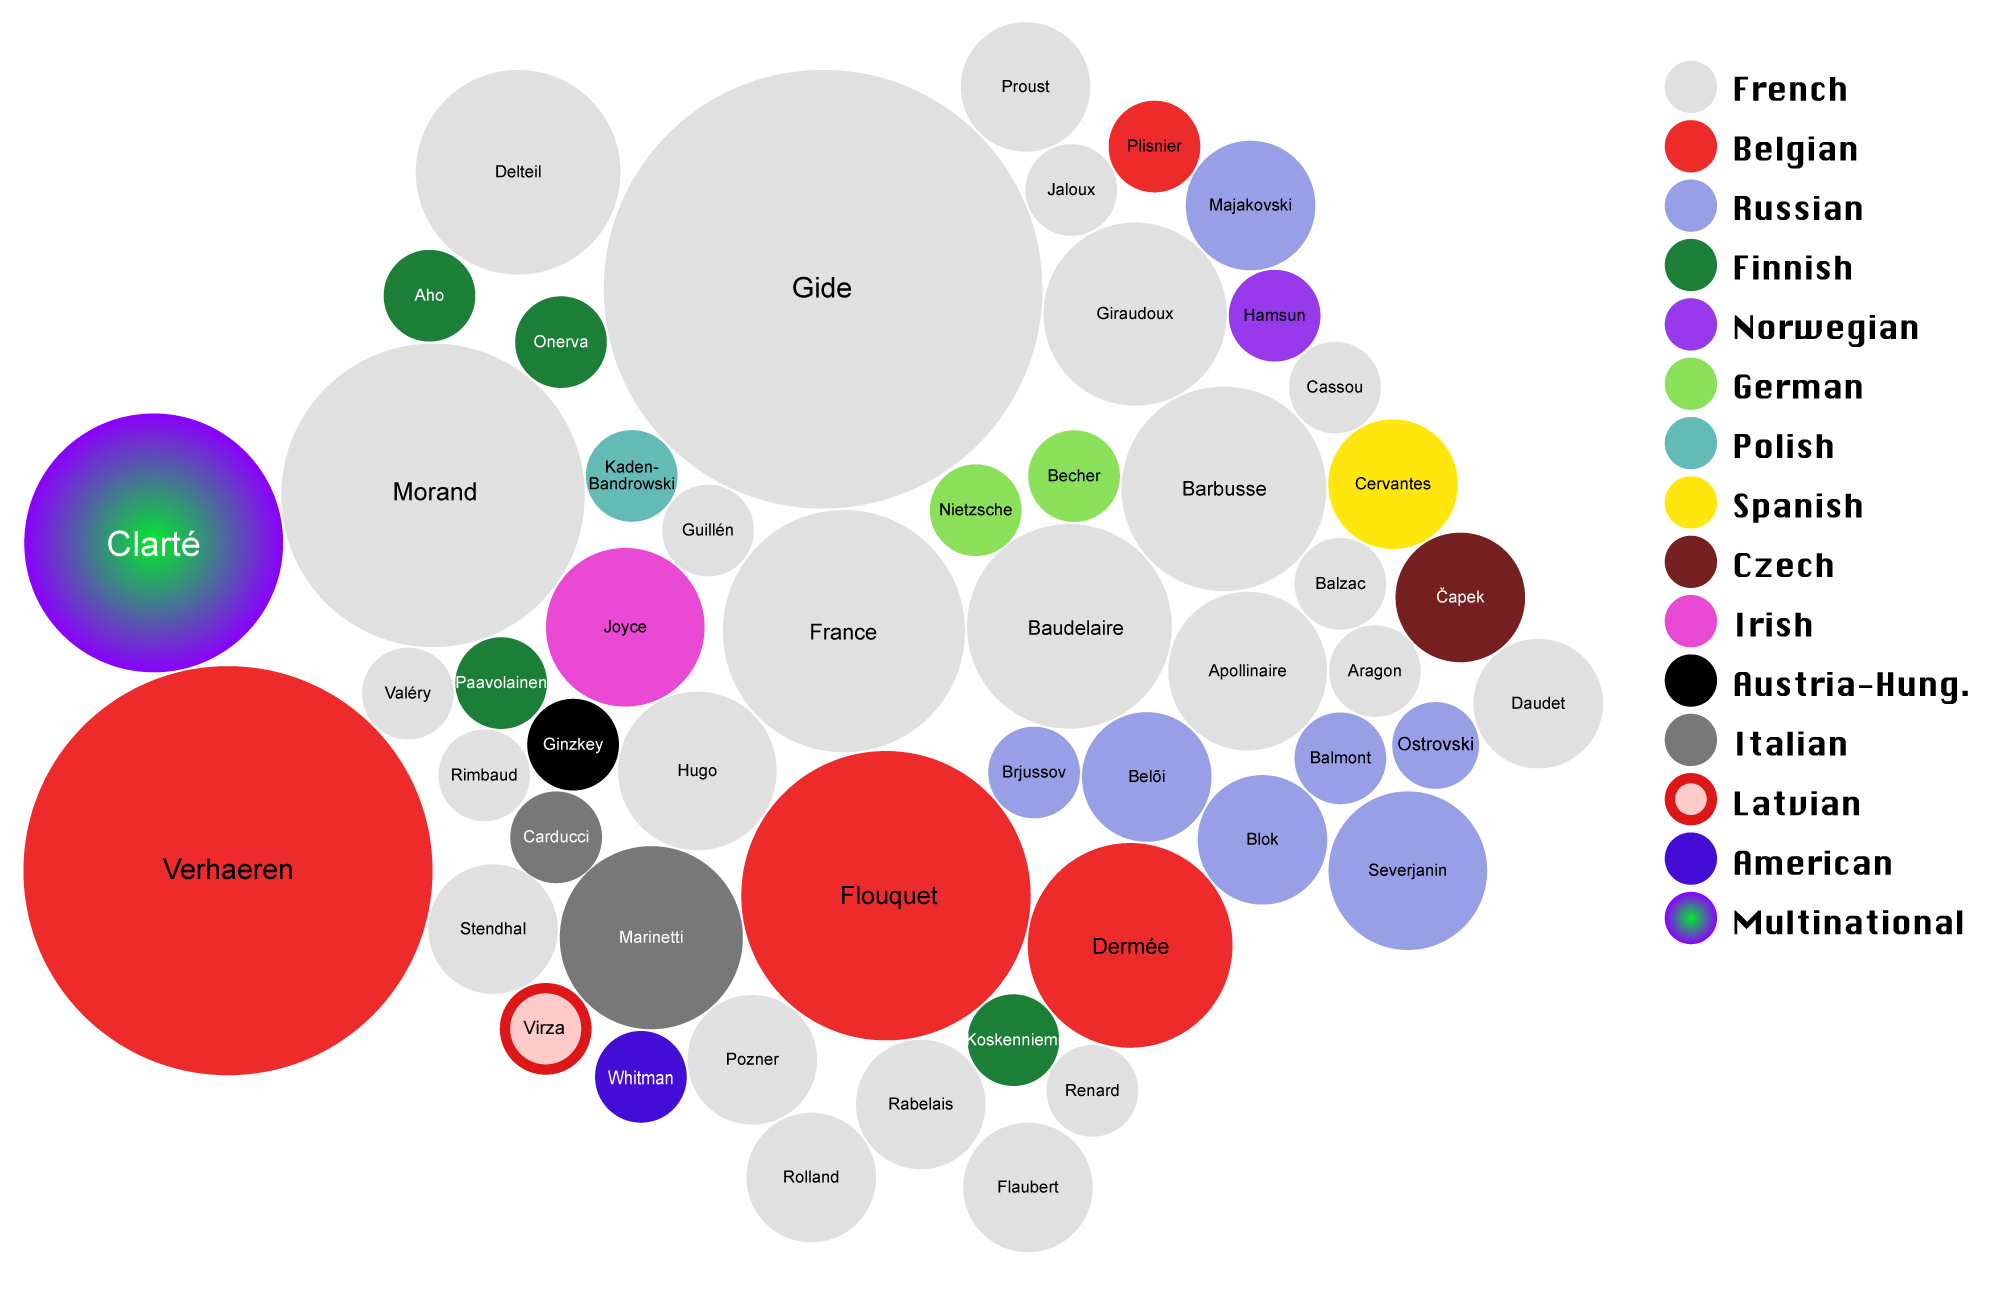
\includegraphics[width=\textwidth]{mummud}
  \caption{Foreign writers and countries mentioned in the correspondence based on the proper name index.  The size of the circle depends on the number of occurences in the corpus.}
  \label{fig2}
\end{figure}


KORP search allows us to see the concordances of the Gide mentions, their absolute and relative frequency in the corpus, but not only. KORP allows us to organise the statistics by all the categories used in the corpus, including metadata categories. To know who of the authors and when mentioned Andre Gide, we only have to add those metadata categories (``sender'' and ``date'') to the statistics criteria; other metadata and linguistic categories can also be used for more sophisticated statistics that is connected to the concordances and broader context text blocks. 

\begin{table}
\caption{Statistics of mentioning Gide in KORP, organised by word form, sender and date.}\label{tab1}
\begin{tabular}{| l | l | l | r|}
  \hline
  word & sender & date & Total\\
  \hline
  Gide'i & Semper & -- & 6.4 (2)\\
  Gide'i & Semper & 1926-12-13 & 3.2 (1)\\
  Gide'i & Semper & 1928-05-26 & 3.2 (1)\\
  Gide'il & Barbarus & 1928-05-26 & 3.2 (1)\\
  Gide'i & Semper & 1929-04-03 & 3.2 (1)\\
  Gide & Semper & 1929-05-06 & 3.2 (1)\\
  Gide'i-raamatule & Semper & 1929-04-03 & 3.2 (1)\\
  Gide'i & Semper & 1929-10-29 & 3.2 (1)\\
  Gide' & Semper & 1929-11-10 & 3.2 (1)\\
  Gide'i & Barbarus & 1929-12-08 & 3.2 (1)\\
  Gide & Semper & 1930-01-10 & 3.2 (1)\\
  Gide'i & Semper & 1930-10-13 & 3.2 (1)\\
  Gide'i & Barbarus & 1930-10-19 & 3.2 (1)\\
  Gide'i & Semper & 1931-07-03 & 3.2 (1)\\
  \hline
  &&Total:&51.5 (16)\\
\hline
\end{tabular}
\end{table}


From the statistics we see that it was mainly Semper who talked about Gide and the time interval is 1926 to 1930. It aligns well with the literary history: in 1928 Semper graduated as Master of Arts from the University of Tartu (with a master’s diploma in literary studies, “The structure of the literary style of Andr\'e Gide”) and continued his work at the university as an aesthetics and stylistics lecturer. 

\section{Future work / Perspectives}

Application of corpus linguistic methods in literary studies requires meticulous preparation of the material and transforming it into a text corpus. The text corpus of the correspondence of the writers, translators and friends Johannes Semper and Johannes Barbarus allows to go further with two different directions:

Firstly, to pose principally new type of research  questions, e.g according to the networks of  writers or ideas influenced  the original works of the both authors…..


KORP helps to analyse these arguments, presented by Estonian literary scholars in the 1970s:
1) The correspondence of Semper and Barbarus is subjective and emotional, the letters reveal the character and state of mind of the authors at the moment of writing them.
2) The letters demonstrate the authors’ awareness of topical problems in Estonia and in Europe.
3) The subject range of the letters includes everyday life, health, hobbies (hunting, swimming, skating, etc.), visits and visitors, literary work, books and reading, and the literary, economic and political life in Estonia and Europe.


Using the Semper \& Barbarus correspondence, we will study how such abstract semantic research problems can be clarified with the help of corpus linguistic methods and KORP.

Such archival materials as a private correspondences of writers have a great cultural value, but promise an incredible linguistic importance as well. The elaborated search possibilities of KORP may be used to verify objectively, via linguistic analysis, the conclusions which have so far been drawn by using traditional methods of literary research, mainly using the well known method of slow close reading of the texts. 



%
% ---- Bibliography ----
%
% BibTeX users should specify bibliography style 'splncs04'.
% References will then be sorted and formatted in the correct style.
%
\bibliographystyle{splncs04}
\bibliography{laaketal}
%
\end{document}
